\subsection{Twitter analysis}
Between January 1st, 2010, and September 23rd, 2021, we are able to retrieve 4285 tweets with keyword “Cameroon flood” and 213 tweets with keyword “Cameroun inondation” (Figure \ref{fig:timeevolutioncumulation}). Dates with rapid increase in cumulative number of tweets are likely related to local flooding events. The largest outbursts for the number of tweets are in September 2012 and August 2015. The event in September 2012 seemed to be related to actual flood events in Cameroon, while the event in August 2015 was related to flood events in Nigeria as a resulting of water releases from a major dam in Cameroon. 

Analyzing the interactions between tweets using number of likes, number of retweets, and number of replies, we found that the interactions with each tweet vary over 3 orders of magnitudes. 95\% of all tweets have less than 5 likes, while the tweet with the largest number of likes has 778 likes. This reflects that some users have a much larger influence to the public that others.

Using tf-idf vectorization, we found the following words to be among the common words: “dam”, “Nigeria”, “releases”, “alert”, “water”, “issues”, “disaster”, “warning”, “kill”. We have also generated word clouds using the most common words for both keyword “Cameroon flood” and “Cameroun inundation” (Figure \ref{fig:Wordclouds}). 

\begin{figure}[hbt!]
	\centering
	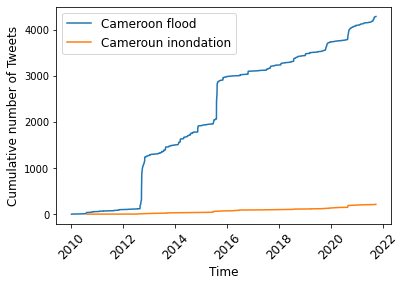
\includegraphics[width=0.8\linewidth]{figure/timeevolutioncumulation.png}
	\caption{Time evolution of the cumulative number of tweets retrieved using the keywords “Cameroon flood” and “Cameroun inondation”}
	\label{fig:timeevolutioncumulation}
\end{figure}

\begin{figure}[htp]
	\centering
	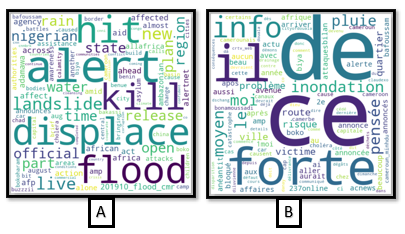
\includegraphics[width=0.8\linewidth]{figure/Wordclouds.png}
	\caption{Word clouds generated from content in the tweets retrieved using the keywords “Cameroon flood” (A) and “Cameroun inundation” (B)}
	\label{fig:Wordclouds}
\end{figure}


With the processed texts, the sentimental analysis reveals that about half of the tweets are neural in polarity. Among those that are not neural, 60\% shows positive polarity and 40\% shows negative polarity. In terms of subjectivity of the texts, we found an average subjectivity of 0.22 (see Figure \ref{fig:Sentimentalanalysis}). Since this value is closer to 0 than 1, this means that the texts are generally more objective than subjective. Since the content is generally more factual rather than opinions, it is not unexpected that the sentimental of the majority of tweets turns out to be closer to neutral.

We also manually analyzed the content in the tweets in French retrieved using the keyword “Cameroun inundation” between February 17 \textsuperscript{th}, 2018, and May 31\textsuperscript{st}, 2021. We found tweet content on 19 days that are related to flooding events in Douala, Cameroon (see Table \ref{table:twitteranalysis2020}). Among these, 4 days (July 25\textsuperscript{th}, 2018, August 21\textsuperscript{st}, 2020, August 22\textsuperscript{nd}, 2020, August 24\textsuperscript{th}, 2020) show significantly higher number of tweets per day. 

Most of the tweets on flooding events in Douala are almost evenly distributed among jokes, alert, sensitization and information. Some tweets are complaints (11\%) and very few calls to action mentioned (see Figure \ref{fig:twitteranalysis2020}). Floods from July 25th, 2020 , August 21st, 2020, and August 24th, 2020 recorded the highest number of tweets (5 to 14 tweets/day).
Analysis of the descriptive statistics of the tweets shows that in Cameroon, people are tweeting about floods, but the number of tweets is still very low compared to the statistics of tweets about other natural disasters in developed countries (e.g., hurricanes, floods, fires). Moreover, most of the tweets are not alerts or direct mentions on flood management. Therefore, there is a need to use social media more constructively so that an increasing number of Twitter users communicate about floods to improve flood predictability, registration, and response.


\begin{figure}[hbt!]
	\centering
	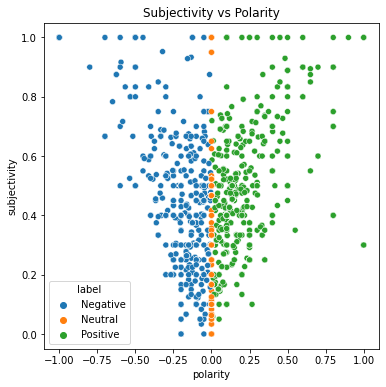
\includegraphics[width=0.8\linewidth]{figure/Sentimentalanalysis.png}
	\caption{Sentimental analysis of tweets with keyword “Cameroon floods”. The tweets are classified based on polarity as negative (polarity < 0, blue), neural (polarity = 0, orange), and positive (polarity > 0, green)}
	\label{fig:Sentimentalanalysis}
\end{figure}

\begin{table}[hbt!]\centering
\begin{tabular}{llll}
\hline
N° & Date       & N° & Date       \\
\hline
1  & 17/02/2018 & 11 & 04/09/2019 \\
2  & 04/03/2018 & 12 & 03/07/2020 \\
3  & 25/07/2018 & 13 & 21/08/2020 \\
4  & 26/07/2018 & 14 & 22/08/2020 \\
5  & 02/11/2018 & 15 & 24/08/2020 \\
6  & 30/06/2019 & 16 & 27/08/2020 \\
7  & 17/07/2019 & 17 & 04/09/2020 \\
8  & 07/08/2019 & 18 & 15/09/2020 \\
9  & 10/08/2019 & 19 & 31/05/2021 \\
10 & 23/08/2019 &    &  \\
\hline        
\end{tabular}
\caption{\label{table:twitteranalysis2020} Flood dates in Douala from Tweets record from February 2018 to may 2021}
\end{table}


\begin{figure}[hbt!]
	\centering
	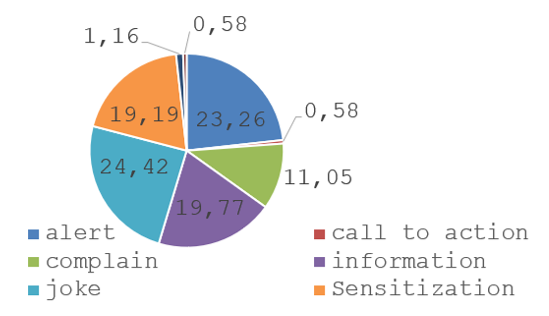
\includegraphics[width=0.8\linewidth]{figure/twitter_analysis_2020.png}
	\caption{Narrative of Twitter message screening in 2020}
	\label{fig:twitteranalysis2020}
\end{figure}
